\chapter{Część sprzętowa} 

\section {Schemat blokowy multipleksera SWD oraz jego użycia}

Rysunek \ref{SWD_multiplexer block diagram} przedstawia schemat blokowy multipleksera. Składa się on z poniższych bloków:
\begin{enumerate}
    \item STM32F103C8 MCU - mikrokontroler odpowiedzialny za sterowanie pozostałymi częściami multipleksera SWD i komunikację z komputerem
    \item szereg diod - wskaźniki obecnie wybranego urządzenia docelowego
    \item wtyczka 20 pin w standardzie ARM JTAG
    \item szereg multiplekserów analogowych 1 do 8 - szczegółowy schemat na rysunku \ref{mux_matrix diagram}
    \item 16 wtyczek do urządzeń docelowych (z powodu zastosowania zarówno standardu pochodzącego z zespołu Bezprzewodowych Sieci Kontrolno-Pomiarowych Katedry Elektroniki AGH (WSN AGH)  jak i CoreSight złącz jest 2 razy więcej niż minimalna wymagana ilość)
\end{enumerate}

 \begin{figure}[H]
    \centering
    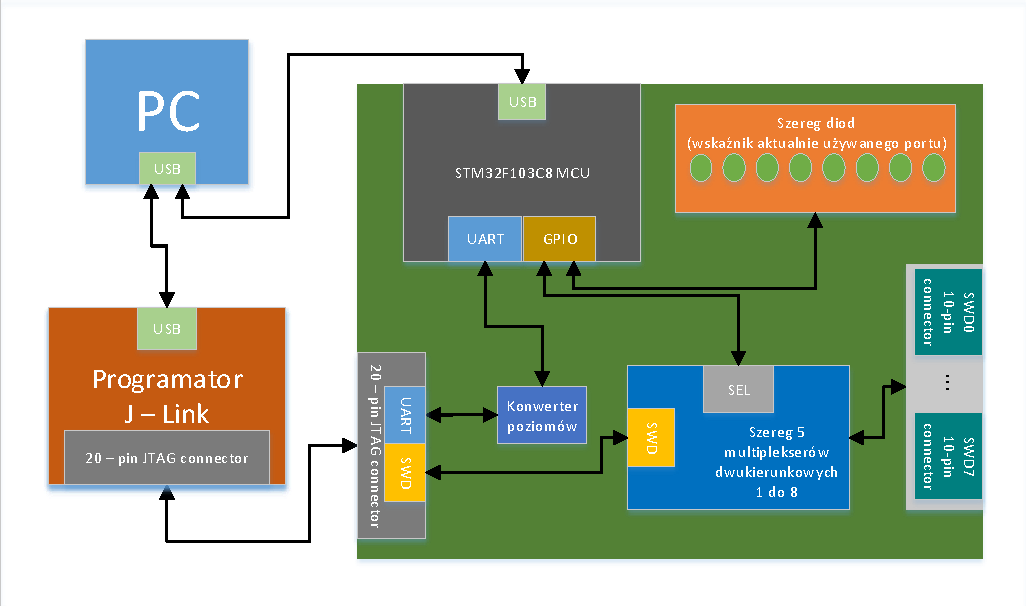
\includegraphics[width=0.75\paperwidth]{images/blokowy_hardware_main.pdf}
    \caption{{Schemat blokowy multipleksera SWD oraz sposób podpięcia urządzeń nadrzędnych.}}
    \label{SWD_multiplexer block diagram}
\end{figure}

 \begin{figure}[H]
    \centering
    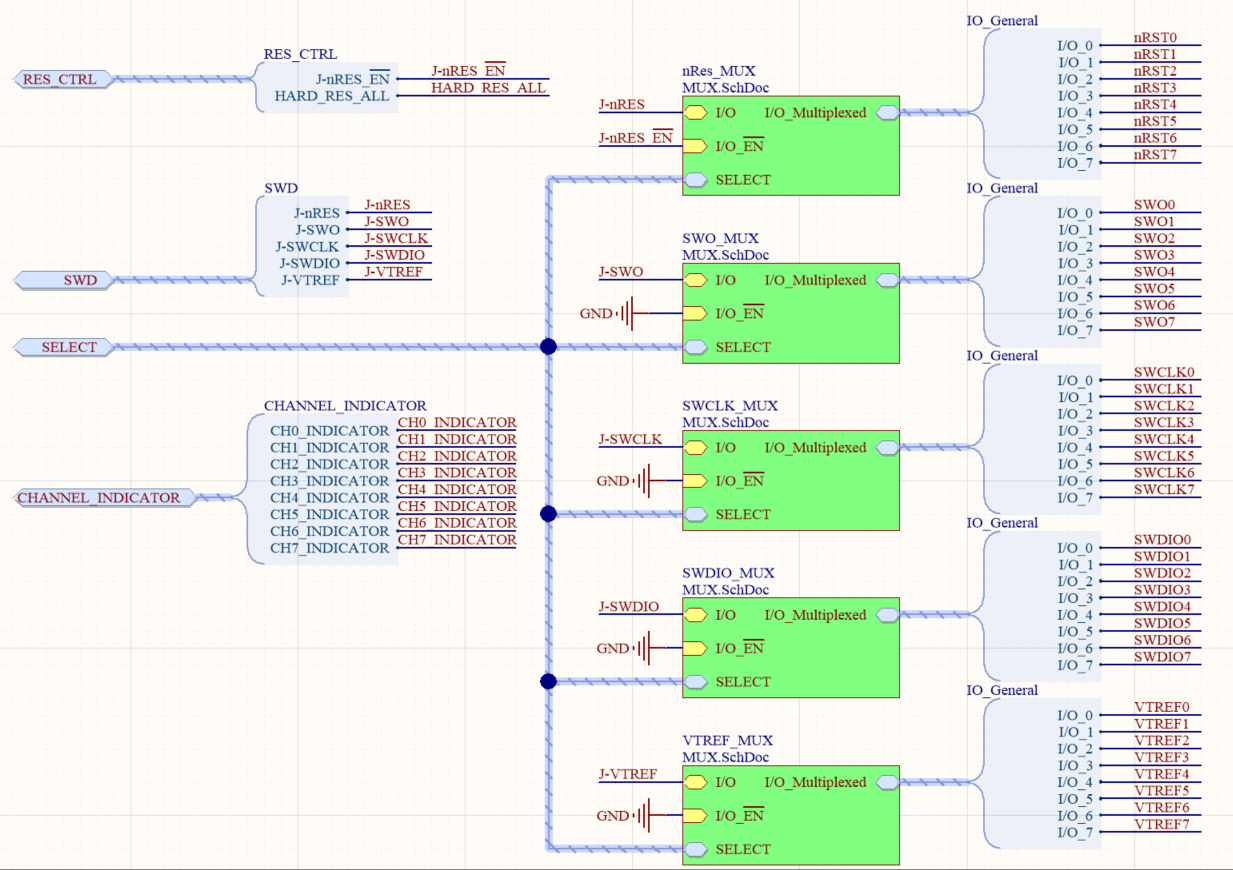
\includegraphics[width=0.8\paperwidth]{images/mux_matrix.png}
    \caption{{Schemat szczegółowy szeregu 5 multiplekserów dwukierunkowych.}}
    \label{mux_matrix diagram}
\end{figure}

Na rysunku \ref{mux_matrix diagram} znajduje się szczegółowy schemat wewnętrzny bloku \enquote{Szereg 5 
multiplekserów 
dwukierunkowych 1 do 8} z rysunku  \ref{SWD_multiplexer block diagram}.
Pokazuje on sposób połączenia multiplekserów analogowych przełączających linie sygnałowe interfejsu SWD. Bloki o nazwie zakończonej na \enquote{MUX} posiadają wewnętrzny schemat na rysunku \ref{SN74CBT3251_connection}.
Magistrala \enquote{RES\_CTRL} steruje włączeniem multipleksera \enquote{nRes\_MUX}, co z kolei pozwala na opięcie sygnału reset z programatora i sterowanie nim w każdym urządzeniu docelowym poprzez tranzystor zwierający ten sygnał do masy (Tranzystor ten poziada oznaczenie Q1 na ryzunku \ref{target_connectors}).


\section{Sekcja zasilania}
Układ zasilany jest z portu USB lub z programatora. Wymaga to użycia diod (D9 i D10 na schemacie), które zabezpieczałyby przed zwarciem w przypadku podłączenia na raz obu źródeł zasilania. Zasilacz podaje kolejno napięcia:
\begin{enumerate}
    \item 5 V, niestabilizowane\\
    Linia 5 V używana jest do zasilania multiplekserów analogowych, oraz stabilizatorów liniowych dla linii 3.3 V oraz 1.8 V. Schemat na rysunku \ref{5V_power_supply}
    \begin{figure}[H]
    \centering
    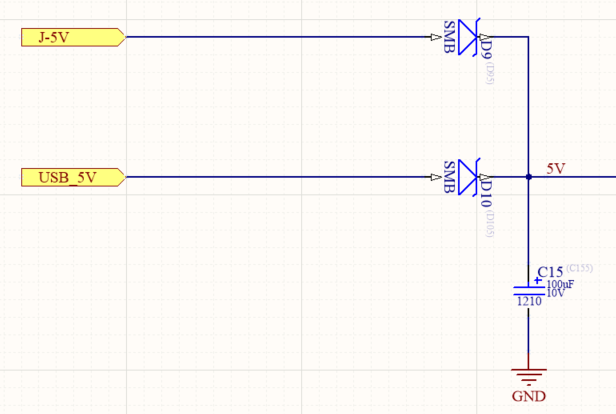
\includegraphics[width=0.35\paperwidth]{images/5V_supply.png}
    \caption{sekcja 5 V zasilacza}
    \label{5V_power_supply}
    \end{figure}

    \item 3.3 V, stabilizowane \\
    Linia ta jest używana do zasilania mikrokontrolera STM32F103C8, oraz służy jako jedno z napięć odniesienia dla konwertera stanów logicznych. Z tego źródła zasilana jest dioda "Power" wskazująca włączenie urządzenia.
    Schemat na rysunku \ref{3.3V_power_supply}
    
    \begin{figure}[H]
    \centering
    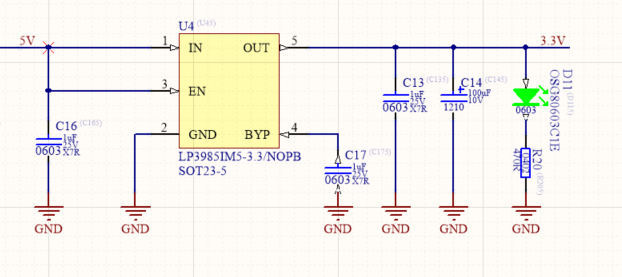
\includegraphics[width=0.55\paperwidth]{images/3,3V_supply.png}
    \caption{sekcja 3.3 V zasilacza}
    \label{3.3V_power_supply}
    \end{figure}
    
    \item 1.8 V, stabilizowane\\
    To źródło zasilania służy jedynie jako źródło napięcia 1.8V dla jednego z konwerterów stanów logicznych.  
    Schemat na rysunku \ref{1.8V_power_supply}
    
    \begin{figure}[H]
    \centering
    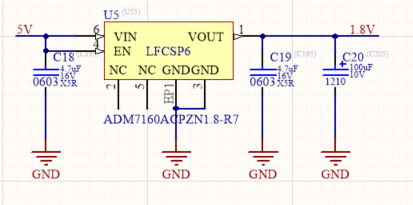
\includegraphics[width=0.45\paperwidth]{images/1,8V_supply.png}
    \caption{sekcja 1.8 V zasilacza}
    \label{1.8V_power_supply}
    \end{figure}
    
\end{enumerate}

\section{Realizacja sprzętowa interfejsów komunikacyjnych USB i UART}

Programator J-Link, który może zostać użyty jako urządzenie sterujące poprzez interfejs UART, dostosowuje poziomy wejściowe i wyjściowe interfejsów do napięcia referencyjnego (napięcie zasilania urządzenia docelowego.) Z racji faktu iż multiplekser SWD zaprojektowany jest pod kątem urządzeń pracujących z napięciami zasilania od 1.8V do 5V, J-Link nie będzie pracował jedynie na napięciu 3.3 V (jest to napięcie zasilania mikrokontrolera osadzonego na płycie multipleksera SWD). Tworzy to potrzebę konwersji poziomów dla samego interfejsu UART. Wygodny do takich zastosowań jest układ TXS0102YZPR, konwertujący poziomy logiczne. Układ ten ma jednak ograniczenie polegające na tym, że jedno z wejść musi mieć zagwarantowany wyższy bądź równy poziom napięcia odniesienia. W tym projekcie tak by nie było, gdyż, urządzenia docelowe mają pracować pomiędzy 1.8 V a 5V. Rozwiązaniem problemu było dodanie dodatkowego stopnia przejściowego na napięciu 1.8 V. Dlatego właśnie w projekcie użyto dwóch układów TXS0102YZPR.
Ogólne i szczegółowe schematy połączeń konwerterów poziomów znajdują się na rysunkach \ref{UART_level_shifters} oraz \ref{level shifter component sheet}

\begin{figure}[H]
    \centering
    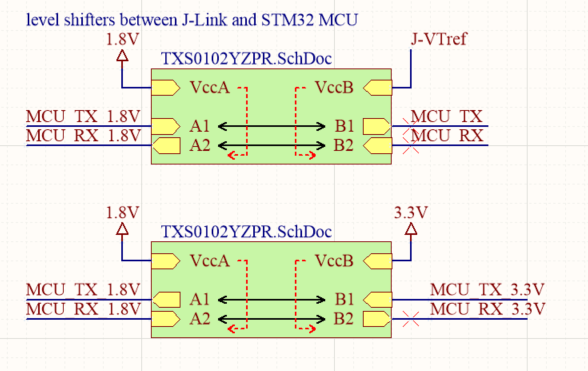
\includegraphics[width=0.55\paperwidth]{images/MCU_level_shifters.png}
    \caption{schemat blokowy układu konwerterów poziomów logicznych}
    \label{UART_level_shifters}
\end{figure}

\begin{figure}[H]
    \centering
    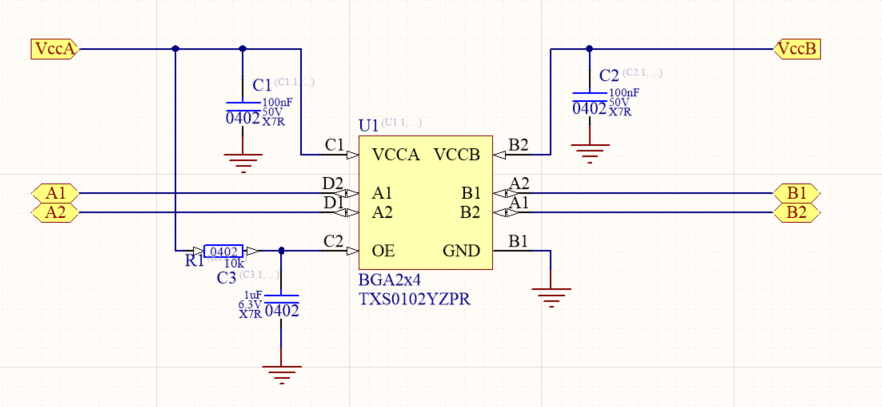
\includegraphics[width=0.55\paperwidth]{images/level_shifter_component_sheet.png}
    \caption{schemat podłączenia  układu $TXS0102YZPR$}
    \label{level shifter component sheet}
    \end{figure}

\section{Problem różnych napięć zasilania urządzeń docelowych}
Możliwość działania do 8 urządzeń docelowych pracujących w różnych standardach napięcia dla stanu wysokiego wymaga użycia sygnału zwrotnego napięcia referencyjnego (celem przekazania go do programatora). W takim wypadku niezbędne jest użycie analogowego multipleksera, gdyż przenosi on sygnał na zasadzie połączenia, nie zmieniając przy tym wartości napięcia. Sygnał SWDIO jest ponadto sygnałem dwukierunkowym, dlatego najłatwiejszym sposobem jego przełączania jest użycie multipleksera analogowego. Nic nie stoi na przeszkodzie użycia takich samych multiplekserów na pozostałych liniach sygnałowych.

\section{Multipleksacja sygnałów}
Przełączanie sygnałów zostało zrealizowane poprzez pięć multiplekserów analogowych $SN74CBT3251$ firmy Texas Instruments. Układ ten został wybrany ze względu na odpowiednio niskie czasy propagacji sygnału. (tabela \ref{tab:mux_propagation_table}) Wymaganie to jest konieczne, aby spełnić zapotrzebowanie na szybkozmienne sygnały celem przyspieszenia debugowania lub wgrywania oprogramowania do pamięci mikrokontrolera docelowego. Ma to znaczenie zwłaszcza w przypadku aż ośmiu urządzeń docelowych. Zasilanie takiego układu nie jest bardzo wymagające - zmiany tego napięcia wpływają jedynie na szybkość propagacji.

\begin {table}[H]
\begin{center}
\begin{tabular}{ |c|c|c|c|c|c| } 
\hline
parametr & Z (wejście) & Do (wyjście) & Vcc &  max & jednostka\\
\hline
\multirow{1}{*}[-7.5pt]{czas propagacji} & \multirow{1}{*}[-7.5pt]{A lub B} & \multirow{1}{*}[-7.5pt]{B lub A} & $Vcc = 4 V$          & $0.35$ & ns\\
&                       &      & $Vcc = 5 V \pm 0.5 V$  & $0.24$ & ns\\ 
\hline
\multirow{1}{*}[-7.5pt]{czas propagacji} & \multirow{1}{*}[-7.5pt]{S} & \multirow{1}{*}[-7.5pt]{A} & $Vcc = 4 V$          & $6$ & ns\\
&                       &      & $Vcc = 5 V \pm 0.5 V$  & $5.5$ & ns\\ 
\hline
\multirow{1}{*}[-7.5pt]{czas aktywacji} & \multirow{1}{*}[-7.5pt]{S} & \multirow{1}{*}[-7.5pt]{B} & $Vcc = 4 V$          & $6.4$ & ns\\
&                       &      & $Vcc = 5 V \pm 0.5 V$  & $5.8$ & ns\\ 
\hline
\end{tabular}
\caption{Parametry propagacyjne multipleksera analogowego $SN74CBT3251$ . Źródło:\cite{SN74CBT3251_datasheet_propagation}}
\label{tab:mux_propagation_table}
\end{center}
\end {table}

\begin{figure}[H]
    \centering
    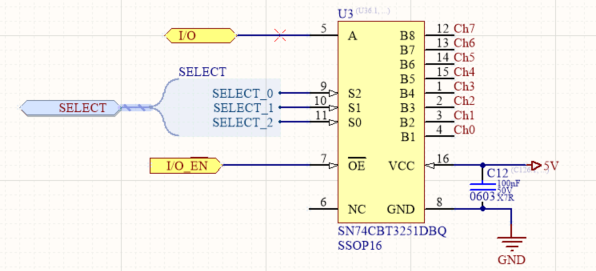
\includegraphics[width=0.6\paperwidth]{images/MUX_connection.png}
    \caption{Schemat połączenia multipleksera analogowego $SN74CBT3251$.}
    \label{SN74CBT3251_connection}
\end{figure}

Na schemacie można zobaczyć błąd powstały podczas projektowania obwodu sterowania multiplekserem. Sygnały SELECT\_0 i SELECT\_2 zostały omyłkowo podłączone na odwrót. Problem ten jednak został wykryty i poprawiony na etapie testów. Błędne działanie zostało skorygowane poprzez podmianę zachowań wyprowadzeń GPIO w oprogramowaniu.


\section{Zabezpieczenia przeciwprzepięciowe i przeciwzakłóceniowe}
Każde z wyjść multiplekserów zabezpieczone jest dolnoprzepustowymi filtrami przeciwzakłóceniowymi i przeciwprzepięciowymi. Ma to na celu uniknięcie uszkodzenia multipleksera z w przypadku wystąpienia krótkotrwałego potencjału wyższego niż 5V pochodzącego od strony urządzeń docelowych (np. dotknięcie wyprowadzeń dłonią naładowanego elektrycznie użytkownika - ESD). Filtrację tę wykonają układy scalone $EMI5208MUTAG$. Każdy z nich filtruje po 8 linii sygnałowych.

 \begin{figure}[H]
    \centering
    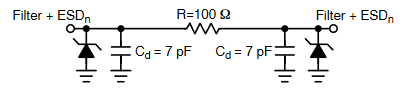
\includegraphics[width=0.7\paperwidth]{images/EMI5208MUTAG_internal_schematic.png}
    \caption{Schemat wewnętrzny filtra $EMI5208MUTAG$ . Źródło:\cite{EMI5208MUTAG_datasheet}}
    \label{EMI5208MUTAG_internal_schematic}
\end{figure}

 \begin{figure}[H]
    \centering
    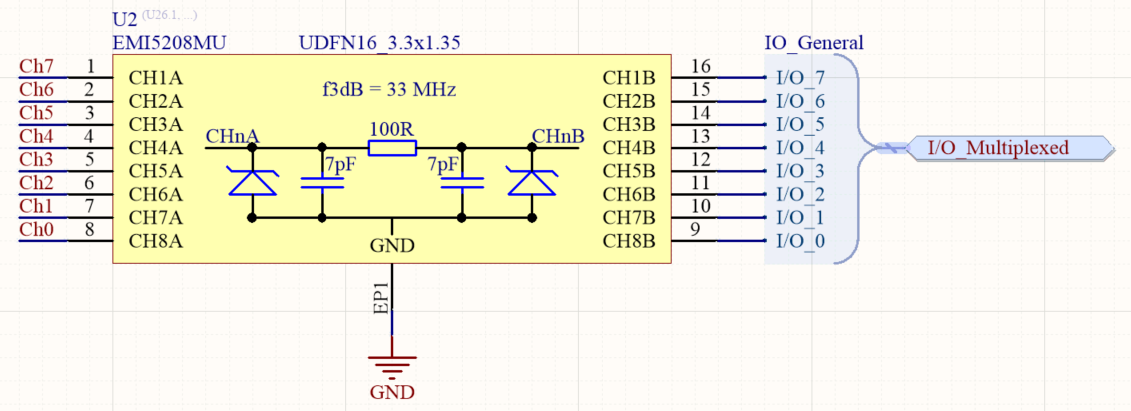
\includegraphics[width=0.7\paperwidth]{images/EMI_connection.png}
    \caption{Schemat połączenia filtra $EMI5208MUTAG$ .}
    \label{EMI5208MUTAG_connection diagram}
\end{figure}


Zabezpieczony został także port mini USB. Dla osiągnięcia bezproblemowego połączenia, użyty został dedykowany temu zastosowaniu układ scalony: USBLC6-2SC6. Układ ten oparty jest na pięciu diodach transil, które gwarantują zabezpieczenie zarówno linii zasilającej jak i dwóch linii danych zapewniając przy tym transmisję USB 2.0 high speed (480Mb/s).
Jednocześnie układ zapewnia niski pobór pasożytniczego prądu (do 150 nA) oraz niewielką pojemność pasożytniczą (maksymalnie 3.5 pF).

\begin{figure}[H]
    \centering
    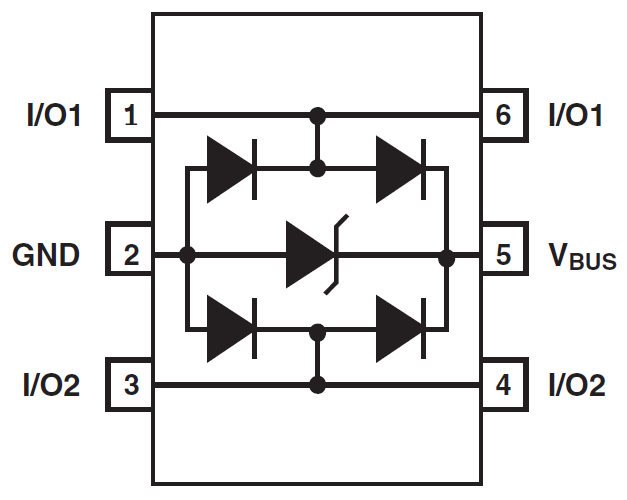
\includegraphics[width=0.45\paperwidth]{images/USBLC6-2SC6_internal_schematic.png}
    \caption{Schemat wewnętrzny filtra $USBLC6-2$ . Źródło:\cite{USBLC6-2_datasheet}}
    \label{USBLC6-2SC6_internal_schematic}
\end{figure}


\begin{figure}[H]
    \centering
    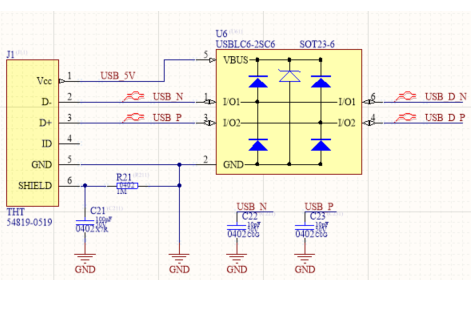
\includegraphics[width=0.8\paperwidth]{images/USB_ESD_protection2.png}
    \caption{Schemat połączenia filtra $USBLC6-2$ i gniazda mini USB.}
    \label{USBLC6-2SC6_connection}
\end{figure}

\section {Przyciski}
Przyciski to przełączniki typu tactswitch. (rysunek \ref{tactswitches}) Celem uproszczenia oprogramowania zdecydowano o eliminacji wpływu zjawiska drgania styków sposobem sprzętowym poprzez zastosowanie kondensatorów gaszących oscylacje.

\begin{figure}[H]
    \centering
    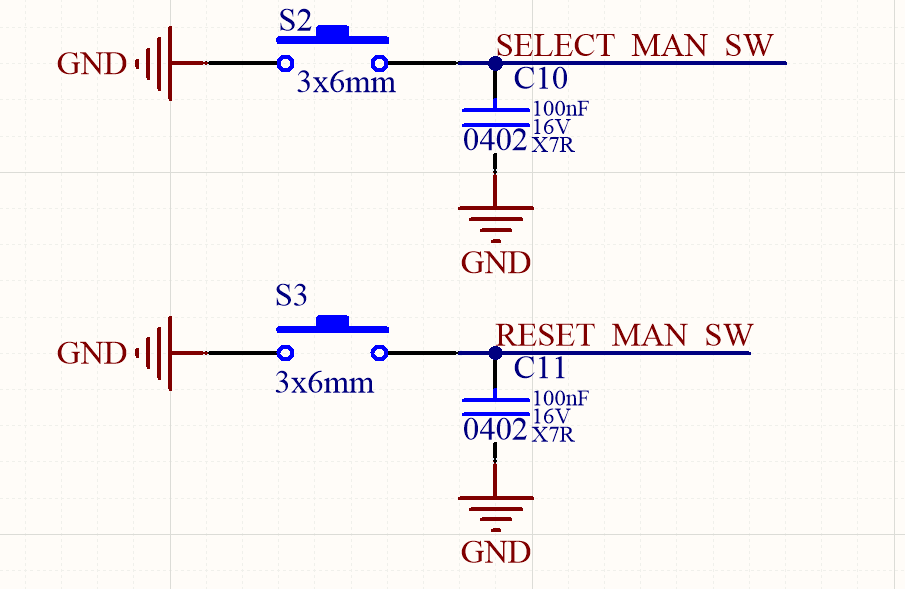
\includegraphics[width=0.7\paperwidth]{images/MCU_switches_debouncing.png}
    \caption{Schemat połączenia przycisków.}
    \label{tactswitches}
\end{figure}


\section{Gniazda zastosowane do podłączenia urządzeń docelowych}

Do podpięcia urządzeń docelowych użyto dwóch rodzajów gniazd. Wynika to z wymaganej zgodności z urządzeniami docelowymi zaprojektowanymi dotychczas w zespole Bezprzewodowych Sieci Kontrolno-Pomiarowych Katedry Elektroniki AGH (złącza bez plastikowej otoczki, rysunek \ref{WSN_Connector}) oraz pełnej kompatybilności z urządzeniami docelowymi wykorzystującymi standard CoreSight 10. Dodatkowo rozszerzono funkcjonalność gniazd zgodnych ze standardem CoreSight10 o wyprowadzenia portu szeregowego UART w miejscu klucza, który nie jest podpięty do żadnego sygnału, oraz w miejsce pinu nieużywanego w trybie SWD. (rysunek \ref{CoreSight10_capable_Connector}) W trybie zgodności z J-TAG pin ten służył jako sygnał TDI. 
Złącza interfejsu UART z gniazd prowadzących do urządzeń docelowych zostały wyprowadzone na złączach szpilkowych o rozstawie 2.54 mm. (złącze oznaczone jako P4 na rysunku \ref{target_connectors}) Ma to na celu możliwość podpięcia zewnętrznego monitora portu szeregowego.


\begin{figure}[H]
  \centering
  \begin{minipage}[b]{0.4\textwidth}
    \centering
    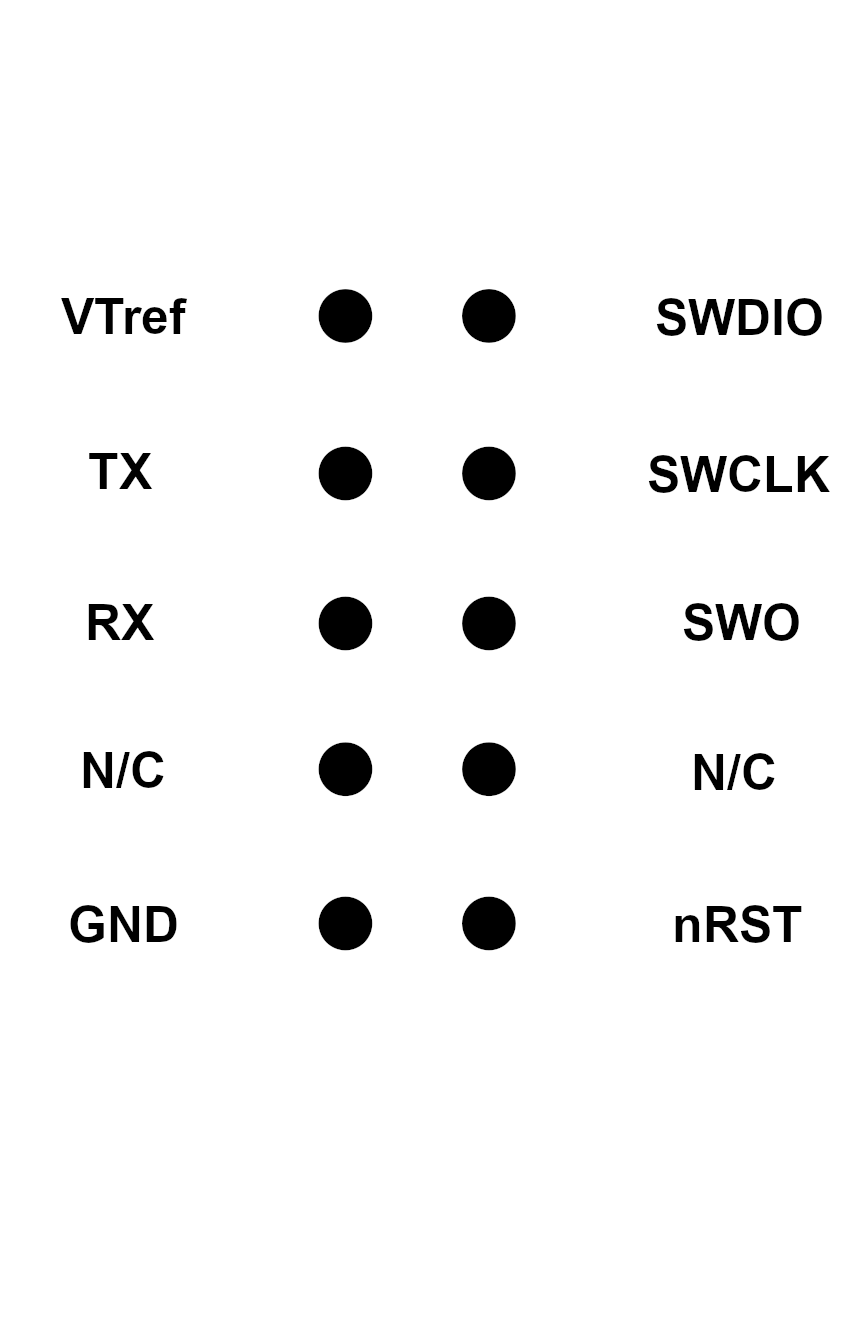
\includegraphics[height=0.4\paperwidth]{images/WSN_plug.png}
    \caption{Schemat wyprowadzeń wtyczki opracowanej w WSN AGH.}
    \label{WSN_Connector}
  \end{minipage}
  \hfill
  \begin{minipage}[b]{0.4\textwidth}
    \centering
    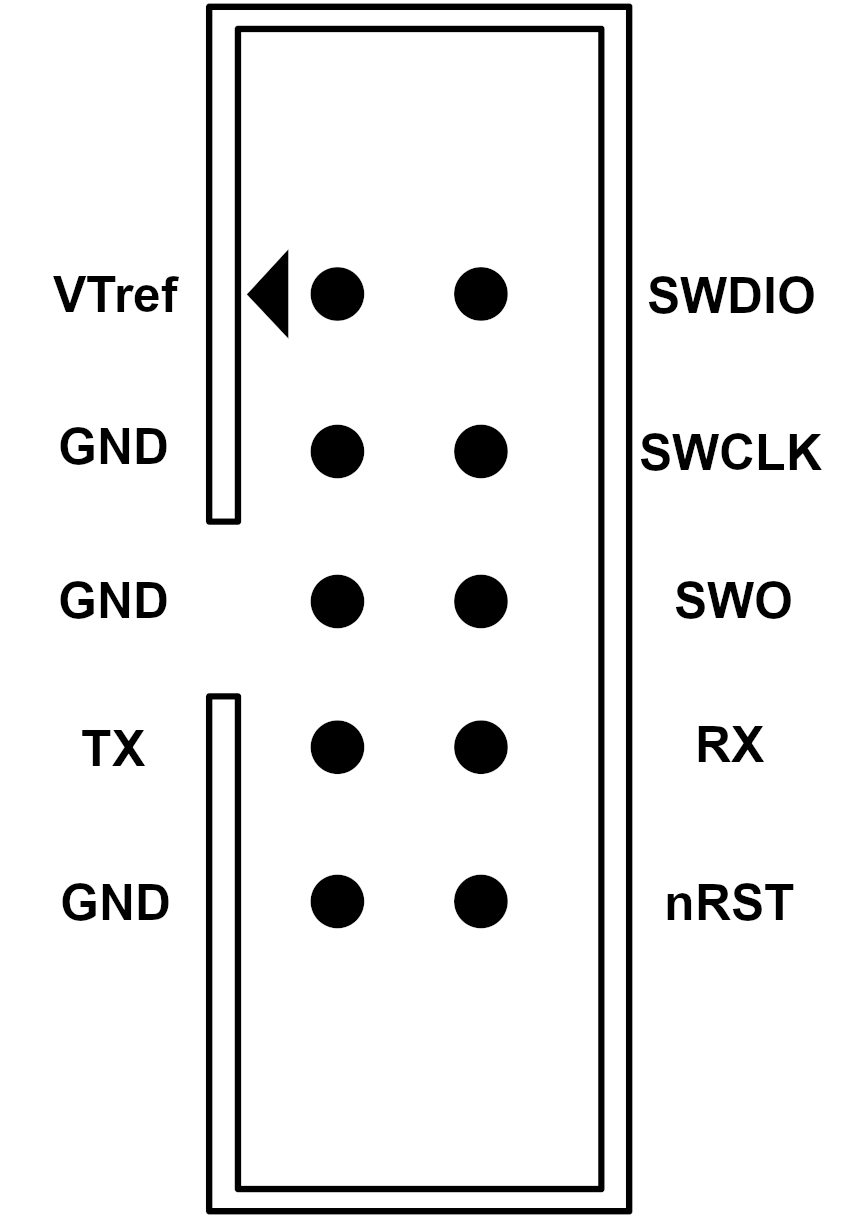
\includegraphics[height=0.4\paperwidth]{images/CoreSight10.png}
    \caption{Schemat wyprowadzeń wtyczki zgodnej z CoreSight10. Źródło:\cite{CoreSight10_documentation} }
    \label{CoreSight10_capable_Connector}
  \end{minipage}
\end{figure}

\begin{figure}[H]
    \centering
    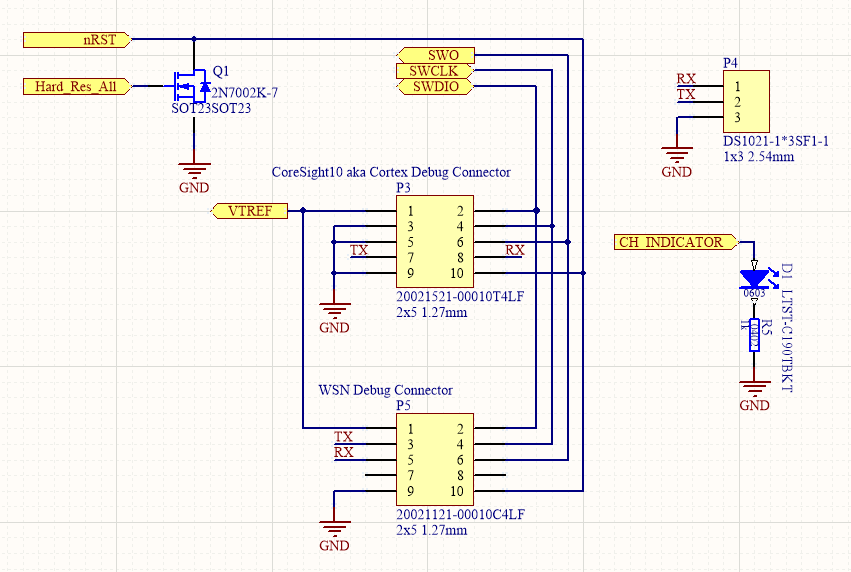
\includegraphics[width=0.75\paperwidth]{images/target_connectors.png}
    \caption{Schemat połączenia wyprowadzeń gniazd w stronę urządzenia docelowego.}
    \label{target_connectors}
\end{figure}



\section{Połączenie wyprowadzeń mikrokontrolera}

W projekcie użyto  mikrokontrolera STM32F103C8. To popularny mikrokontroler posiadający między innymi interfejs USB, który nie wymaga dodatkowego układu scalonego odpowiedzialnego za konwersję interfejsów. Pomaga to zaoszczędzić miejsce na płycie PCB oraz zminimalizować koszty produkcji urządzenia. Mikrokontroler zawiera wbudowaną pętlę PLL, która pozwala uzyskać częstotliwość taktowania zegara procesora do 72MHz przy rezonatorze wykorzystującym kryształ kwarcowy o częstotliwości oscylacji 16MHz.

\begin{figure}[H]
    \centering
    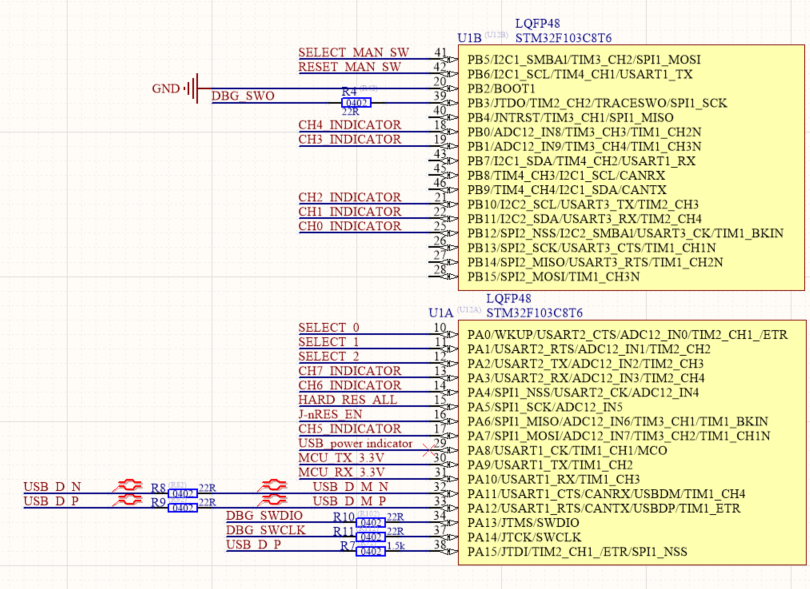
\includegraphics[width=0.65\paperwidth]{images/MCU_STM32.png}
    \caption{Schemat połączenia wyprowadzeń mikrokontrolera STM32F103C8 odpowiedzialnych za urządzenia wejścia-wyjścia}
    \label{MCU_STM32}
\end{figure}

\begin{figure}[H]
    \centering
    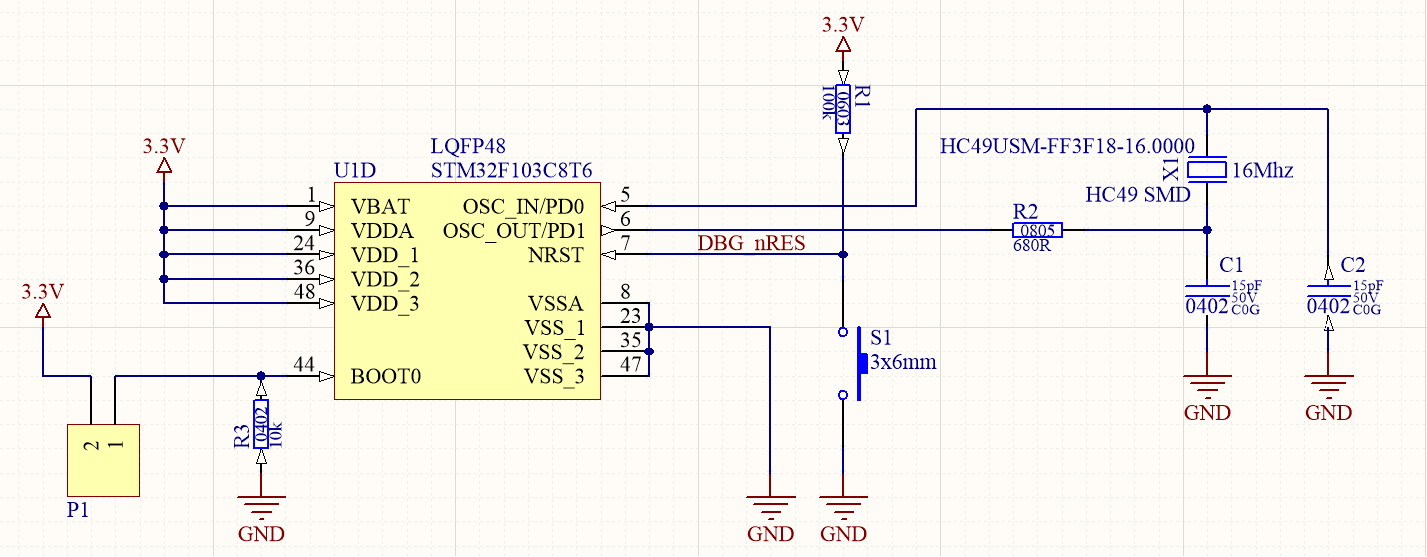
\includegraphics[width=0.65\paperwidth]{images/MCU_oscillator_and_reset.png}
    \centering
    \caption{Schemat połączenia wyprowadzeń mikrokontrolera STM32F103C8 odpowiedzialnych za resetowanie i układ rezonatora}
    \label{MCU_STM32_osc_and_reset}
\end{figure}

